% \PassOptionsToPackage{table}{xcolor}
\documentclass[11pt]{beamer}
\usepackage[utf8]{inputenc}
\usepackage[english]{babel}
\usepackage{amsmath}
\usepackage{amsfonts}
\usepackage{amssymb}
\usepackage{graphicx}
\usepackage{tikz}
\usepackage{algorithm}
\usepackage{algorithmic}
\usepackage{silence,lmodern}
\usepackage{csquotes}
\usepackage[backend=bibtex, bibencoding=ascii, style=authoryear, doi=false, isbn=false,url=false, uniquename=init, giveninits=true]{biblatex}
\usepackage{multimedia}
\usepackage{dirtytalk}
\usepackage{pgfplotstable,booktabs,longtable}
\usepackage{grffile}
\usepackage{marvosym} % color image
\WarningFilter{biblatex}{Patching footnotes failed}


% \mode<presentation>
% {
    \usetheme[hideothersubsections]{PaloAlto}
    % \usecolortheme{beaver}
% }
\usetikzlibrary{calc,trees,positioning,arrows,chains,shapes.geometric,
decorations.pathreplacing,decorations.pathmorphing,
shapes,matrix,shapes.symbols,plotmarks,decorations.markings,
shadows,shapes.geometric,arrows}

\setbeamercolor{logo}{bg=white}  %controls the color of the logo area
\setbeamerfont{footnote}{size=\tiny}

% \addbibresource{library.bib}

\makeatletter
\setlength{\beamer@headheight}{.9cm}
\makeatother

\author{S M Al Mahi}
\title[ECEN-5283 Computer Vision]{Project 5: \\Object Detection\\Gibbs and Metropolis Sampling}
\setbeamercovered{transparent} 
\setbeamertemplate{navigation symbols}{}


\logo{
\includegraphics[width=1cm]{Oklahoma_State_University_logo.png}}
\institute{Oklahoma State University} 
\date{\today} 
\subject{}
\begin{document}

\setbeamertemplate{sidebar left}{}
\begin{frame}
\titlepage
\end{frame}

\newpage

\setbeamertemplate{sidebar left}[sidebar theme]
\section{Project Objective}
\begin{frame}
\frametitle{Project Objective}
	\begin{block}{Objectives}
	\begin{enumerate}
		\item Implement Jump Diffusion Markov Chain Monte Carlo(JD-MCMC) methods
    \item Implemented Gibbs and Metropolis sampling
		\item Apply them for object detection in image
		\item Analyze the result with different parameter and test cases
	\end{enumerate}
	\end{block}
\end{frame}


\section{Background}
\begin{frame}
\frametitle{Back Ground: MCMC}
	\begin{block}{Objectives}
	\begin{enumerate}
		\item MCMC is used for efficiently generate a set of discrete samples to approximate the underlying unknown distribution
    	\item Sample proposal is made
		\item Sample is evaluated and then rejected or accepted based on a likelihood  function
	\end{enumerate}
	\end{block}
\end{frame}

\section{Background}
\begin{frame}
\frametitle{Back Ground: Model Order}
	\begin{block}{Objectives}
	\begin{enumerate}
		\item MCMC methods like Important sampling and Gibbs sampling assumes the model order to be known
    	\item In Object detection project we want to estimate model order $K^*$
		\item JD-MCMC assumes the model order estimation as a Markov chain where states are the model orders
		\item Where transition function is the ratio posterior probabilities of two neighboring state
		\item The model order estimation is the stationary state of the Markov Chain
	\end{enumerate}
	\end{block}
\end{frame}

\begin{frame}
\frametitle{Back Ground: Model Order}
	\begin{block}{Objectives}
	\begin{enumerate}
		\item MCMC methods like Important sampling and Gibbs sampling assumes the model order to be known
    	\item In Object detection project we want to estimate model order $K^*$
		\item JD-MCMC assumes the model order estimation as a Markov chain where states are the model orders
		\item Where transition function is the ratio posterior probabilities of two neighboring state
		\item The model order estimation is the stationary state of the Markov Chain
	\end{enumerate}
	\end{block}
\end{frame}

\begin{frame}
\begin{figure}
  \frametitle{JD-MCMC: Algorithm}
  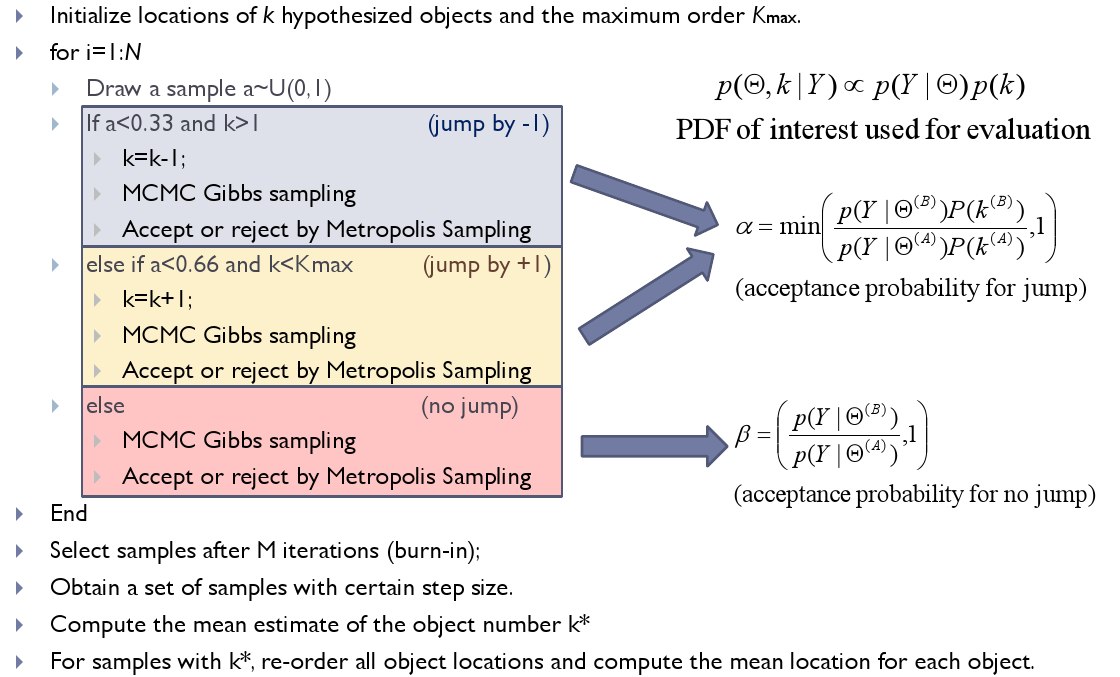
\includegraphics[width=.9\textheight]{JD-MCMC.png}
  \caption{Random}
\end{figure}
\end{frame}

\begin{frame}
\begin{figure}
  \frametitle{JD-MCMC: Final Output}
  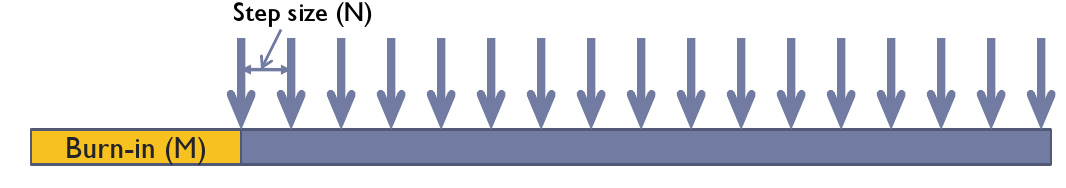
\includegraphics[width=.9\textheight]{Final.png}
  \caption{Random}
\end{figure}
\end{frame}

\begin{frame}
\frametitle{Observations}
	\begin{itemize}
		\item The JD-MCMC algorithm have two phases; Jump and Diffusion
    	\item In the jump phase we induced prior knowledge about model order $k^*$ using Poission distribution parameter $\lambda$
		\item We have run the experiment using good and bad priors by setting the $\lambda$
		\item The initial model order $k^*$ is set as $k^*=\lambda +2$
		\item We have found that all the test cases the object detection locks on all the objects correctly
		\item The model order also converges to the correct model order.
		\item We will show the result for some of the test cases throughout the following slides
		\item The Videos for objection and model order estimation processes have been attached with the slides
	\end{itemize}
\end{frame}


% ------------------------------------------------------------------------------------------------------------
\begin{frame}
\frametitle{Test Case 1: Iteration N=50, Burn In M=10}
\begin{columns}
\begin{column}{.45\textwidth}
\begin{figure}
  \includegraphics[width=.9\textwidth]{good/discs1_initial.png}
  \caption{Initial}
\end{figure}
\end{column}
\begin{column}{.45\textwidth}
\begin{figure}
  \includegraphics[width=.9\textwidth]{good/discs1_final.png}
  \caption{Final}
\end{figure}
\end{column}
\end{columns}
\end{frame}

\begin{frame}
\frametitle{Test Case 2: N=50, M=10}
\begin{columns}
\begin{column}{.45\textwidth}
\begin{figure}
  \includegraphics[width=.9\textwidth]{good/discs2_initial.png}
  \caption{Initial}
\end{figure}
\end{column}
\begin{column}{.45\textwidth}
\begin{figure}
  \includegraphics[width=.9\textwidth]{good/discs2_final.png}
  \caption{Final}
\end{figure}
\end{column}
\end{columns}
\end{frame}

\begin{frame}
\frametitle{Test Case 3: N=50, M=10}
\begin{columns}
\begin{column}{.45\textwidth}
\begin{figure}
  \includegraphics[width=.9\textwidth]{good/discs3_initial.png}
  \caption{Initial}
\end{figure}
\end{column}
\begin{column}{.45\textwidth}
\begin{figure}
  \includegraphics[width=.9\textwidth]{good/discs3_final.png}
  \caption{Final}
\end{figure}
\end{column}
\end{columns}
\end{frame}

\begin{frame}
\frametitle{Test Case 8: N=50, M=10}
\begin{columns}
\begin{column}{.45\textwidth}
\begin{figure}
  \includegraphics[width=.9\textwidth]{good/discs8_initial.png}
  \caption{Initial}
\end{figure}
\end{column}
\begin{column}{.45\textwidth}
\begin{figure}
  \includegraphics[width=.9\textwidth]{good/discs8_final.png}
  \caption{Final}
\end{figure}
\end{column}
\end{columns}
\end{frame}


\begin{frame}
\frametitle{Test Case 12: N=15, M=5}
\begin{columns}
\begin{column}{.45\textwidth}
\begin{figure}
  \includegraphics[width=.9\textwidth]{good/discs12_initial.png}
  \caption{Initial}
\end{figure}
\end{column}
\begin{column}{.45\textwidth}
\begin{figure}
  \includegraphics[width=.9\textwidth]{good/discs12_final.png}
  \caption{Final}
\end{figure}
\end{column}
\end{columns}
\end{frame}

\begin{frame}
\frametitle{Test Case 20: N=15, M=5}
\begin{columns}
\begin{column}{.45\textwidth}
\begin{figure}
  \includegraphics[width=.9\textwidth]{good/discs20_initial.png}
  \caption{Initial}
\end{figure}
\end{column}
\begin{column}{.45\textwidth}
\begin{figure}
  \includegraphics[width=.9\textwidth]{good/discs20_final.png}
  \caption{Final}
\end{figure}
\end{column}
\end{columns}
\end{frame}


\begin{frame}
\frametitle{Test Case 25: N=15, M=5}
\begin{columns}
\begin{column}{.45\textwidth}
\begin{figure}
  \includegraphics[width=.9\textwidth]{good/discs25_initial.png}
  \caption{Initial}
\end{figure}
\end{column}
\begin{column}{.45\textwidth}
\begin{figure}
  \includegraphics[width=.9\textwidth]{good/discs25_final.png}
  \caption{Final}
\end{figure}
\end{column}
\end{columns}
\end{frame}

% ------------------------------------------------------------------------------------------------------------


\section{Challenges and Caveats}
\begin{frame}
\frametitle{Challenges and caveats}
	\begin{itemize}
		\item The likelihood function has some limitations. 
		\item It may produce greater likelihood for wrong model order than better detection with wrong model order.
    	\item Thus the likelihood function is less efficient for model order estimation
		\item However, it is very useful for object detection. Thus in Gibbs Sampling we have used it
		\item For model order estimation the likelihood function should be multiplied by the prior for better model order estimation
		\item Because of the limitation of the likelihood function the prior is very crucial in model order estimation.
		\item Because of clip function object located at the corner and edge of the images are less likely to be detected using trivial approach.
		\item This problem was handled by changing the range for next move of an object using modified range on uniform distribution.
	\end{itemize}
\end{frame}

\begin{frame}
\begin{figure}
  \frametitle{Limitation of Likelihood}
  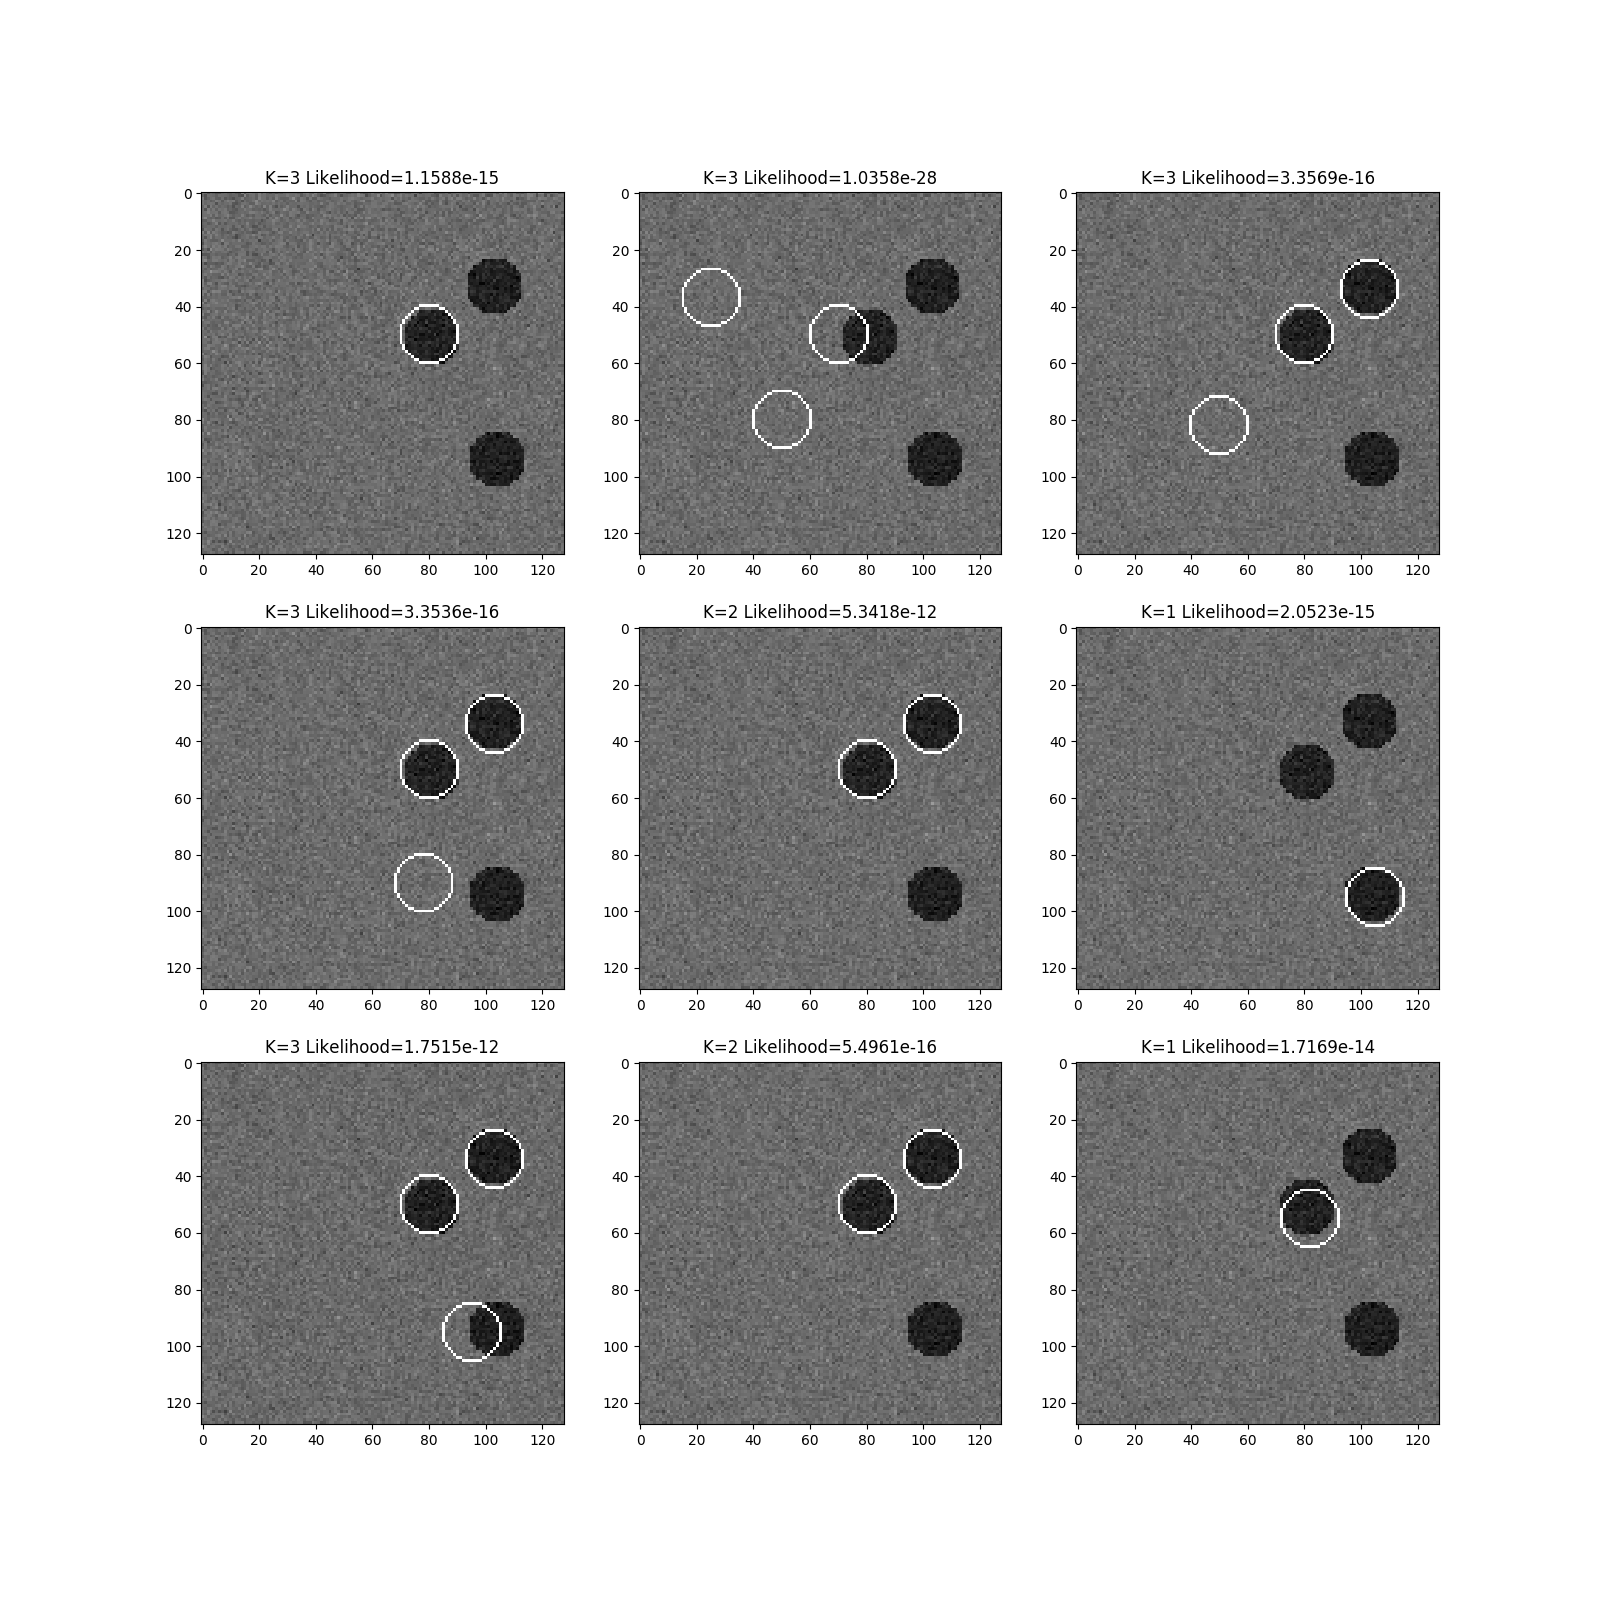
\includegraphics[width=.9\textwidth, height=.8\textheight ]{likelihood_fault.png}
  \caption{Even though the model order of the later one is correct the former produces higher likelihood.}
\end{figure}
\end{frame}

\section{Effects of $\lambda and K^*$}
\begin{frame}
\frametitle{Challenges and caveats}
\begin{columns}
\begin{column}{.45\textwidth}
\begin{figure}
  \includegraphics[width=.9\textwidth]{good/discs12_initial_bad1.png}
  \caption{Initial}
\end{figure}
\end{column}
\begin{column}{.45\textwidth}
\begin{figure}
  \includegraphics[width=.9\textwidth]{good/discs12_final_bad1.png}
  \caption{Final}
\end{figure}
\end{column}
\end{columns}
Finally, we check the effect of choosing a bad $\lambda=18, k^*=3$ for disc 12 test case. 
It totally failed to converge to correct model order even after around double iterations.
\end{frame}

\section{Effects of $\lambda and K^*$}
\begin{frame}
\frametitle{Challenges and caveats}
\begin{columns}
\begin{column}{.45\textwidth}
\begin{figure}
  \includegraphics[width=.9\textwidth]{good/discs12_initial_bad2.png}
  \caption{Initial}
\end{figure}
\end{column}
\begin{column}{.45\textwidth}
\begin{figure}
  \includegraphics[width=.9\textwidth]{good/discs12_final_bad2.png}
  \caption{Final}
\end{figure}
\end{column}
\end{columns}
Finally, we check the effect of choosing a bad $\lambda=3, k^*=25$ for disc 12 test case. 
It totally failed to converge to correct model order even after around double iterations. However,
it locked on the objects correctly which reinforce our assumption that prior has a big role in model order estimation or the jump in JD-MCMC
\end{frame}

% ------------------------------------------------------------------------------------------------------------------

\end{document}

